
\section{Exploración Univariada}\label{univariada}

En esta sección exploro cada índice.Nos vamos a interesar en la población cabecera y la poblacion resto. 


No podemos hacer tabla de frecuencias, entonces sacamos solamente los estadisticos:

% Table created by stargazer v.5.2.2 by Marek Hlavac, Harvard University. E-mail: hlavac at fas.harvard.edu
% Date and time: Fri, Jun 29, 2018 - 8:31:25 PM
\begin{table}[!htbp] \centering 
  \caption{Medidas estadisticas} 
  \label{stats} 
\begin{tabular}{@{\extracolsep{5pt}}lccccc} 
\\[-1.8ex]\hline 
\hline \\[-1.8ex] 
Statistic & \multicolumn{1}{c}{N} & \multicolumn{1}{c}{Median} & \multicolumn{1}{c}{Mean} & \multicolumn{1}{c}{Min} & \multicolumn{1}{c}{Max} \\ 
\hline \\[-1.8ex] 
IDH & 32 & 0.804 & 0.802 & 0.691 & 0.879 \\ 
Población.Cabecera & 32 & 717,197 & 1,196,730.000 & 13,090 & 10,070,801 \\ 
Población.Resto & 32 & 268,111.5 & 360,590.300 & 21,926 & 1,428,858 \\ 
Población.Total & 32 & 1,028,429 & 1,557,320.000 & 43,446 & 10,985,285 \\ 
\hline \\[-1.8ex] 
\end{tabular} 
\end{table} 
\begin{figure}[h]
\centering
\begin{adjustbox}{width=13cm,height=9cm,clip,trim=0cm 0cm 0cm 0cm}
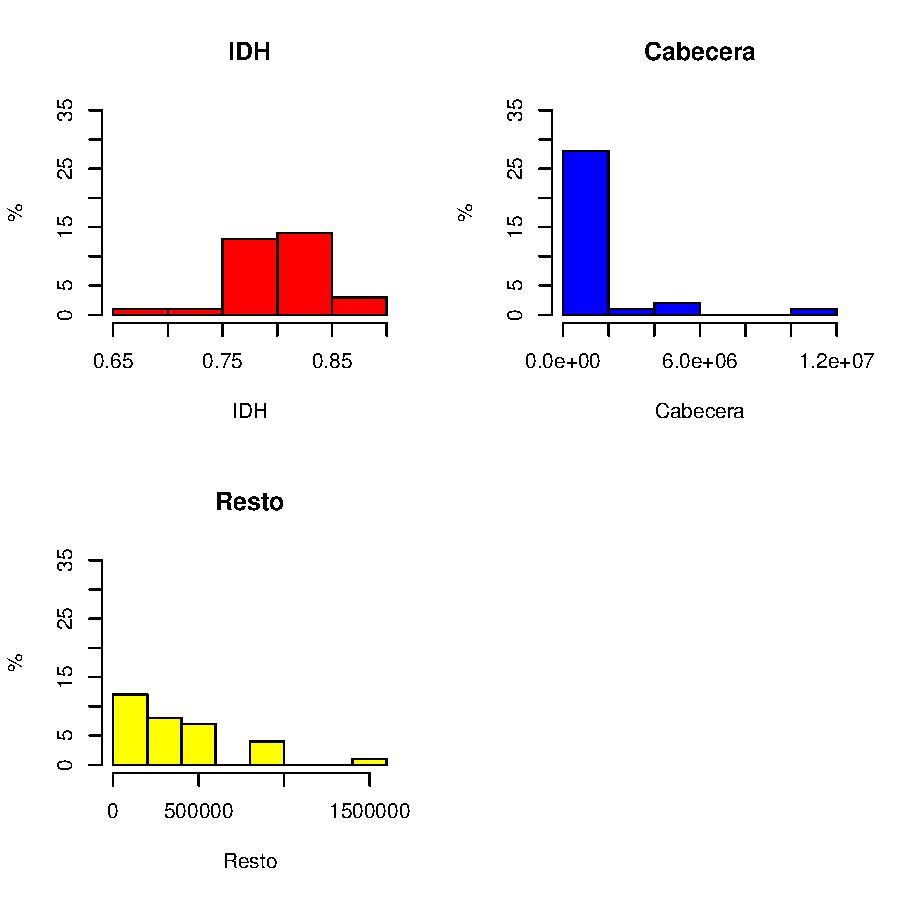
\includegraphics{Proyecto_Final_Univariada-corrPlotX}
\end{adjustbox}
\caption{correlacion entre predictores}
\label{corrPlotX}
\end{figure}

\clearpage

\endinput
